\subsection{Introducción}

	En el trabajo que realizaron Wang et al., los autores identificador el problema que había al detectar y reconocer palabras en imágenes naturales. Ellos identifican, que si bien las actuales aplicaciones de OCR se manejan bien con documentos escaneados, todavía encuentran problemas cuando tratan de procesar texto adquirido en entornos naturales (también referido como texto de escena). Este tipo de texto se ha vuelto más frecuente debido al aumento de dispositivos que son capaces de extraer dicha información, sean estos celulares, tabletas o cámaras.
	
	Durante la competencia de ICDAR (\textit{International Conference on Document Analysis and Recognition}) en 2003, los organizadores tenían como objetivo ver cual era el estado del arte en las diferentes etapas del reconocimiento de texto en escenas naturales. Observaron que habían imágenes con texto que los motores de OCR del momento no podían procesar, por lo tanto, decidieron dividir el problema general que era reconocer palabras en escenas naturales en tres subproblemas:
	
	\begin{itemize}
		\item \textbf{La clasificación de caracteres recortados.}
		
		En este problema se consideran imagenes de caracteres extraidas de escenas naturales. Las imagenes contienen exclusivamente un sólo carácter y sus tamaños se ajustan a las dimensiones del caracter tal como se puede apreciar en la Figura \ref{fig: Caracteres recortados}. El objetivo es identificar qué carácter está reflejado en la imagen a partir de un conjunto predefinido de caracteres que hacen al problema.

		El reconocimiento de caracteres recortados de escenas naturales es un desafio que requiere tener presente algunas cosas. Una de las dificultades de este problema es que algunos caracteres son muy difíciles de dicernir entre sí, por ejemplo, si consideramos las letras mayúsculas y las minúsculas por separado luego una ``Z'' es muy difícil de dicernir de una ``z''. Incluso se puede dar lugar a la confusión entre distintos símbolos, por ejemplo, la ``O'' (letra o mayúscula) y el número ``0'' o el número 6 y la ``G'' (letra ``g'' mayúscula).
						
		Otro elemento que se tiene que tener presente al momento de clasificar caracteres, es el tipo de características locales que se van a obtener de cada imagen. Como se ha explicado en la sección \ref{subsection:feature}, las características son importantes dado que representa los aspectos o cualidades más significativas de un objeto. Si se hace una buena elección de las características locales, se va a ver reflejado en la performance de clasificación.
		
		Las condiciones en que fueron tomadas las imágenes donde se extrajeron los caracteres influye posteriormente en su reconocimiento. Por ejemplo, las variaciones en las condiciones de iluminación, oclusión, posicionamiento al momento de tomar la imagen, etc. Para resolver esto, se puede realizar un pre-procesamiento que ayude a ``limpiar'' la imagen para poder facilitar su reconocimiento posterior.
		
	\begin{figure}[htbp]
		\centering
  		\centerline{ 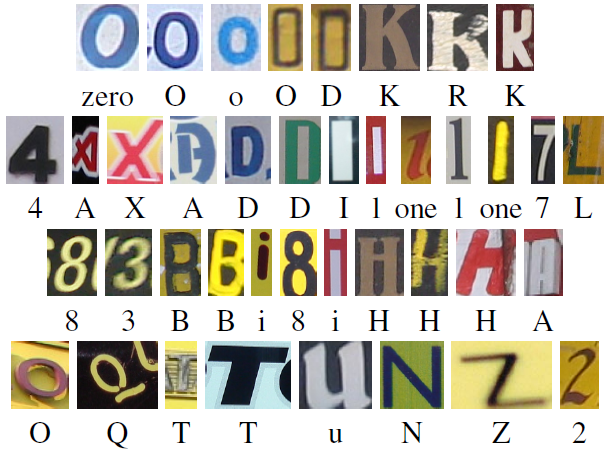
\includegraphics[scale=0.5]{img/hog/confusing_english.png} }
		\caption[Clasificación de caracteres recortados]{Conjunto de caracteres recortados. Imagen extraida del paper de T. E. de Campos et. al. \cite{dCBV09}}
		\label{fig: Caracteres recortados}
	\end{figure}
		
		\item \textbf{Detección de zonas con texto en la imagen.}
		
		Este problema involucra la detección de zonas de la imagen que pueden contener texto. Esto se realiza con el objetivo de priorizar estas regiones en procesamientos posteriores para reducir la complejidad del problema del análisis de texto. La figura \ref{fig: Zona texto} expone un ejemplo de este problema.
		
		Para poder resolver este problema, se debe considerar que las palabras que conforman el texto a detectar, pueden haber sido adquiridas a distintas escalas. Tal es el caso del texto de casi la mayoría de los carteles publicitarios que es posible encontrar en las calles de una ciudad. Otro factor a considerar es la inclinación del texto que puede darse por la posición del observador o por una disposición en el mundo. Además, esta tarea se dificulta si consideramos, al igual que en el reconocimiento de caracteres, las condiciones de la imagen (iluminación, distorsiones, estilo y fuente de las palabras en el texto, etc).
		
		En el trabajo de Chen H. et. al. \cite{ChenH11}, los autores destacan que hay dos categorías al momento de diferenciar las técnicas de reconocimiento de texto. La primera categoría, son las técnicas \textit{basadas en textura} (\textit{texture based} de su traducción al inglés) que destacan al texto como una ``textura'' especial que es distinguible del fondo. Las características se extraen de ciertas regiones de la imagen y se utiliza un clasificador para identificar la existencia de texto. La segunda categoría, son las técnicas basadas en \textit{componentes conectados} (\textit{connected component} de su traducción al inglés), donde se extraen regiones de la imagen y se utilizan restricciones geométricas para descartar candidatos que no sean texto.
		
	\begin{figure}[htbp]
		\centering
		\centerline{ 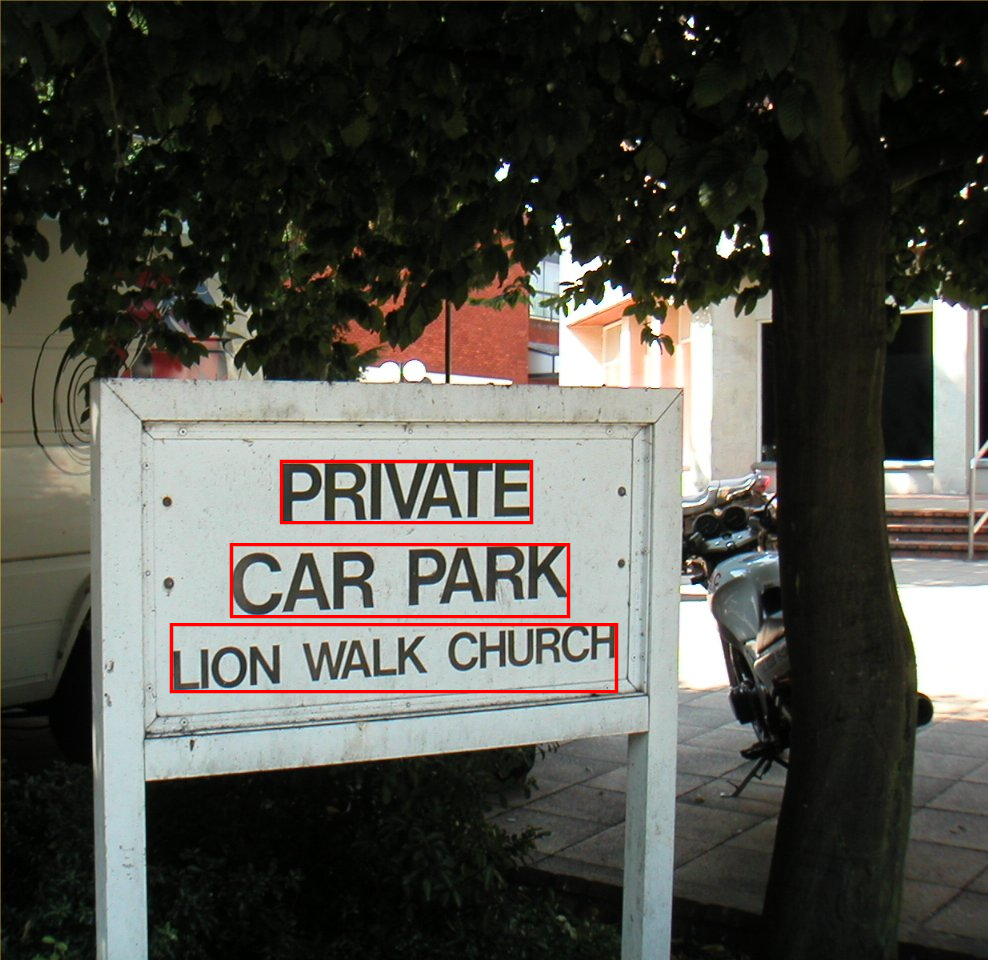
\includegraphics[scale=0.20]{img/zone_with_text.png} }
		\caption[Detección de zonas con texto]{Imagen natural donde las zonas con texto están encasilladas.Imagen tomada del sitio \url{http://libccv.org/post/introducing-ccv-milestone/} }
		\label{fig: Zona texto}
	\end{figure} 
		
		\item \textbf{El reconocimiento de palabras recortadas.}

		En este problema se busca identificar las palabras que se encuentran dentro de las imágenes recortadas. Al igual que el problema del reconocimiento de caracteres, en este problema, cada imagen contiene una sola palabra y la dimensiones de estas imágenes se ajustan a las palabras tal como se puede ver en la Figura \ref{fig: Reconocimiento palabras}.
		
		Una de las dificultades surgen en este problema al manipular imágenes naturales, son las condiciones en que estas fueron adquiridas. Como se explicó anteriormente, las variaciones en la iluminación, la oclusión, entre otros, generan problemas en el reconocimiento. 

		Uno de los métodos que se utiliza en la actualidad y se considera estado del arte son las estructuras pictóricas. Este método fue usado por Wang y Belongie en \cite{WB10}, donde en base a un lexicón (conjunto de palabras), miden la configuración de cada caracter de cada palabra en la imagen. Básicamente toma la ubicación y el puntaje de los caracteres detectados como entrada y encuentra la configuración óptima para una palabra en particular \cite{wang}. Una de las particularidades de este trabajo, es que requiere de un clasificador de caracteres para poder posteriormente realizar el reconocimiento de palabras.
	
	\begin{figure}[htbp]
		\centering
		\centerline{ 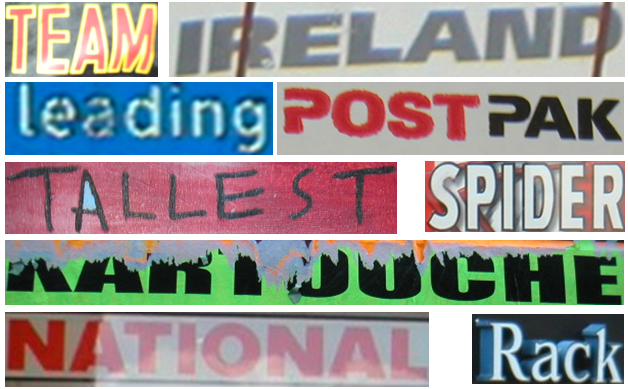
\includegraphics[scale=0.30]{img/cropped_words.png} }
		\caption[Reconocimiento de palabras recortadas]{Conjunto de palabras recortadas de diferentes escenas naturales. Imagen extraida del sitio de \textit{Graphics and Media Lab}, \url{http://graphics.cs.msu.ru/en/science/research/machinelearning/text}}
		\label{fig: Reconocimiento palabras}
	\end{figure}
		
	\end{itemize}

	Dada esta problemática, Wang et al. se enfocaron en un caso especial del reconocimiento de texto de escena donde tenían a disposición un listado de palabras (i.e, un lexicón) para detectar y leer.
		
	Para esto, ellos construyen y evalúan dos sistemas. En el primero, evalúan la performance en la detección y el reconocimiento de palabras de un enfoque con dos etapas que consiste en un detector de texto considerado estado del arte y un destacado motor de OCR. El segundo, es un sistema arraigado en el reconocimiento de objetos genéricos, el cual es una extensión de un trabajo que realizaron anteriormente \cite{WB10}. En \cite{WB10}, los autores consideran a las palabras como categorías de objectos en sí mismas y realizan reconocimiento sobre las categorías de las palabras. Utilizan técnicas propias del reconocimiento de categorías genéricas y las aplican al reconocimiento de palabras. Asi como podemos tener muchas imágenes que representen el objeto ``vehículo'', también es posible aplicar la misma idea para la palabra ``door'' como muestra la Figura \ref{fig: Reconocimiento generico}. La figura representa una analogía al reconocimiento de objetos genéricos.
	
	En \cite{wang}, los autores remarcan que para poder lograr el reconocimiento de palabras en imágenes, es necesario en primera instancia tener un clasificador de caracteres. Este trabajo se enfoca en el reconocimiento de caracteres en ventanas, es decir, imagenes de caracteres recortados de escenas naturales. 
	
	
	
	\begin{figure}[htbp]
		\centering
		\centerline{ 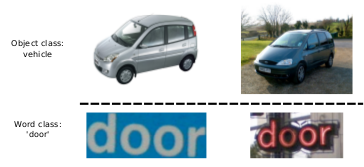
\includegraphics[scale=0.7]{img/object_recognition.png} }
		\caption[Reconocimiento generico de objetos]{Reconocimiento de palabras. Se considera a la palabra como una categoría de objeto al igual que la categoría ``vehiculo'' presentada en la parte superior de la imagen.}
		\label{fig: Reconocimiento generico}
	\end{figure}
